\begin{frame}
    \frametitle{Открытая русскоязычная распределенная система OCR  Shuemacher+}
    \centering
    \begin{block}{Сводная информация}
        \begin{itemize}
            \item Год выполнения: 2024 год
            \item Академический уровень: ВАК
            \item Тема: Обработка данных
        \end{itemize}
    \end{block}  
    
    \begin{block}{Абстракт}
        Shuemacher+ - открытая распределенная система распознания корпусов.
        Модель вычислений описывается классической двуакторской схемой руководитель-рабочий, дополненная
        флагом наличия графического ускорителя. Таким образом,
        руководитель распределяет нагрузку на вычислительные узлы и отрабатывает возникающие
        исключения. 
    \end{block}

\end{frame}


\begin{frame}
    \frametitle{Принципиальная схема распределённых вычислений}
    \centering
    \begin{figure}
        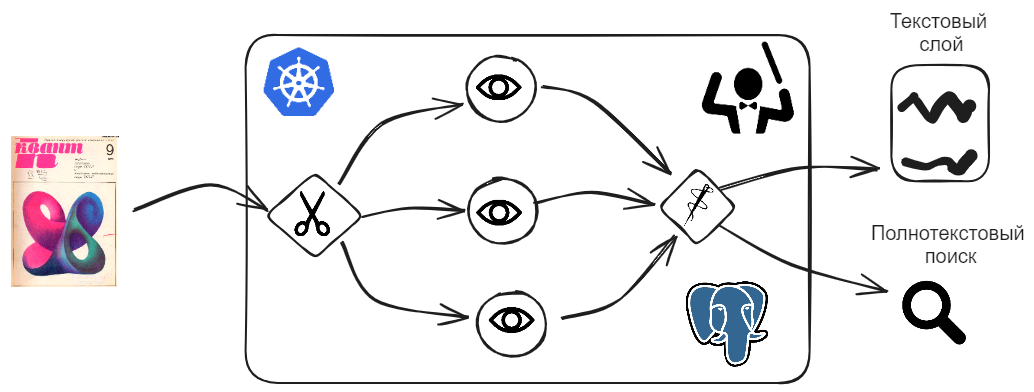
\includegraphics[width=0.9\linewidth]{assets/saga.excalidraw.png}
    \end{figure}
\end{frame}

\begin{frame}
    \frametitle{Схема Монро-Роббинса для клик с суперадитивными факторами}
    \centering
    \begin{block}{Сводная информация}
        \begin{itemize}
            \item Год выполнения: 2025 год
            \item Академический уровень: Q1
            \item Тема: Моделирование
        \end{itemize}
    \end{block}  

    \begin{block}{Абстракт}
        В работе изучается постановка стохастической аппроксимации для супераддитивных функций, оценивающих
        результат совместной деятельности. 
        Изучены и в аналитической форме представлены коэффициенты для функций агрегации mean-max, min-sum и
        квадратичной формы.
    \end{block}
\end{frame}

\begin{frame}
    \frametitle{Исследуемые супераддитивные функции}
    \centering
    \begin{figure}
        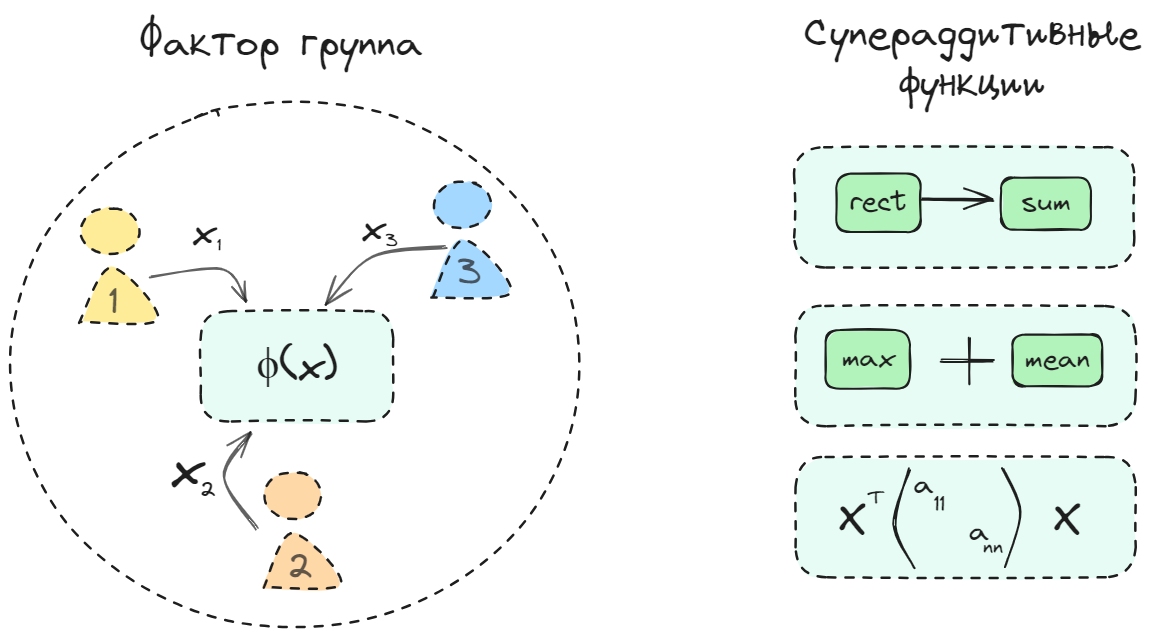
\includegraphics[width=0.9\linewidth]{assets/group.excalidraw.png}
    \end{figure}
\end{frame}


\begin{frame}
    \frametitle{Запись стохастической аппроксимации в форме уравнений Фоккера-Планка}
    \centering
    \begin{block}{Сводная информация}
        \begin{itemize}
            \item Год выполнения: 2025 год
            \item Академический уровень: Q1
            \item Тема: Моделирование
        \end{itemize}
    \end{block}  
    \begin{block}{Абстракт}
        Стохастическая аппроксимация метод поиска корня
        уравнения по случайному несмещенному отклику, аналитическая
        форма которого в общем случае неизвестна. В работе предлагается 
        изучение метода с использованием уравнение Фоккера-Планка, позволяющего задать непрерывно во времени
        оптимальную функцию смещения. 
    \end{block}
\end{frame}

\begin{frame}
    \frametitle{Эволюция распределения инструментальной переменной во времени}
    \centering
    \begin{figure}
        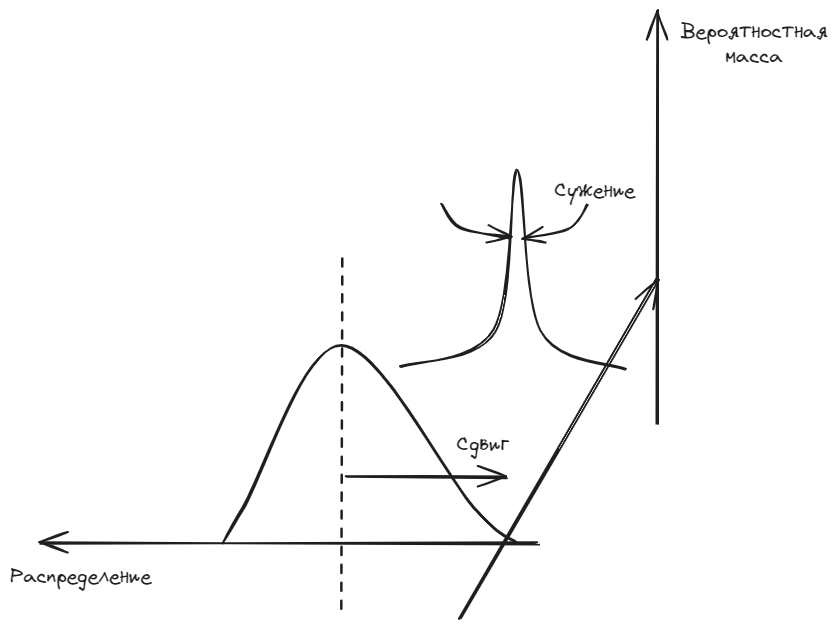
\includegraphics[width=0.85\linewidth]{assets/continious.excalidraw.png}
    \end{figure}
\end{frame}

